\documentclass{bakalarka}
%\usepackage[cp1250]{inputenc}
\usepackage{listings}
\usepackage[utf8]{inputenc} 
\usepackage[czech]{babel}
\usepackage{ae}
\usepackage{fancyhdr}
\usepackage{float}
\usepackage{graphicx}
%\usepackage[pdftex]{graphicx}

\lstset{language=Java,keywordstyle=\color{blue}, commentstyle=\color{Green},stringstyle=\color{red},showstringspaces=false,breaklines=true,tabsize=3,basicstyle=\footnotesize}



\author{Martin Kadlec}
\title{Docházka a výkazy práce pro systém IMIS na platformě Android}
\titlet{}
\titlett{}
\university{Západočeská univerzita v Plzni}
\faculty{Fakulta aplikovaných věd}
\department{Katedra informatiky a výpočetní techniky}
\subject{Diplomová práce}
\town{Plzeň}
\begin{document}
\pagestyle{fancy}
\renewcommand{\chaptermark}[1]{\markboth{\textit{#1}}{}}
\renewcommand{\sectionmark}[1]{\markright{\textit{#1}}{}}
\cfoot{\thepage}
\lhead{\leftmark}
\rhead{\rightmark}
\maketitle
\chapter*{Prohlášení}
\thispagestyle{empty}
Prohlašuji, že jsem bakalářskou práci vypracoval samostatně a výhradně s~použitím citovaných pramenů.
\vskip 1.5em
V Plzni dne \today
\vskip 0.7em
\hskip 9cm Maxipes Fík
\chapter*{Abstract}
\thispagestyle{empty}
Text of abstract.
\pagestyle{empty}
\tableofcontents
\pagestyle{fancy}
\renewcommand{\chaptermark}[1]{\markboth{\textit{#1}}{}}
\renewcommand{\sectionmark}[1]{\markright{\textit{#1}}{}}
\cfoot{\thepage}
\lhead{\leftmark}
\rhead{\rightmark}
\parskip 1em

%\renewcommand{\chaptermark}[1]{\markboth{\textit{#1}}{}}
%\renewcommand{\sectionmark}[1]{\markright{\textit{#1}}{}}
\chapter{Úvod}

\chapter{Současný systém}
IMIS = Integrovaný manažerský informační systém

\section{Oracle forms}
Oracle forms je softwarový produkt vyvinutý společností Oracle. Slouží k vytváření formulářů, které interagují s Oracle databází. Jako programovací jazyk využívá PL/SQL. Produkt byl původně požíval terminálové rozhraní pro komuikaci se serverem. Později byl přepracován do architekrury klient-server.\\ \indent
Prostředí běhu zajišťuje defaultní správu transakcí. Díky tomu je Oracle Forms silný nástroj pro efektivní vývoj aplikací, jejichž primárním cílem je přístup k datům uložených v databázi. 

\paragraph{PL/SQL}
PL/SQL (Procedural Language/Structured Query Language) je procedurální nadstavba jazyka SQL od firmy Oracle založená na programovacím jazyku Ada.

\section{Architektura}
Z hlediska architektury se Oracle Forms aplikace skládá z těchto celků:

\paragraph{Modul formuláře} 
A form (or form module) is the main component that anchors an application and provides the necessary code to interact with the datasource and the user interface. The underlying database data is reflected in multiple items, including fields, check boxes, and radio groups. A form is logically organized into blocks.
\begin{itemize}
\item Datový blok The data block serves as a bridge to the underlying data and provides an abstraction for how the data is reached.
A data block can be associated with a specific database table (or a view), a stored procedure, a FROM clause query, or a transactional triggers. By default, the association between a data block and the database allows for automatic access and manipulation of data in the database.
\item Řídící blok A control block is a block that does not have a relationship to a database table. Control blocks can contain items of any type (buttons, text items, check boxes, etc.), however, regardless of item type, all of the items in a control block are control items--that is, items that do not correspond to columns in a database table.
\end{itemize}

\paragraph{Modul menu} 
The menu module consists of a hierarchy of menus. Each menu consists of the items that can be selected. Menu modules are usually attached to form modules. Every form module has a default menu that includes the commands for all basic database operations, such as insert, update, delete, and query.

\paragraph{Modul PL/SQL knihovny}
The PL/SQL library contains reusable code invoked by other form, menu, or library modules. The code, also called a program unit, can be user-named functions, procedures, or packages. The program unit is stored and executed on the client. The program units are not for database-related code alone. They may contain purely business logic. Libraries make all the PL/SQL code available to the form without being part of the form. The libraries are loaded dynamically. Multiple forms can attach the same PL/SQL library.

\paragraph{Modul knihovny objektů}
Object Library\\
The object-oriented programming concept of reusing code is implemented in Oracle Forms by the object library and PL/SQL library modules. The Object library contains reusable objects and the PL/SQL library contains reusable code.

\begin{figure}[H]
  \centering
  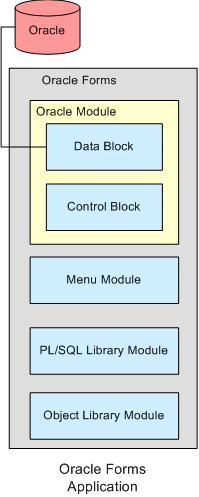
\includegraphics[scale=0.8]{obr/forms_arch3.png}
  \label{}
\end{figure}
TODO obrazek upravit - prepsat Oracle Module na Form Module

\subsection{Triggery}
Aplikace v Oracle pracuje s následujícími typy triggerů:
\begin{itemize}
\item Block-processing triggers: - Block processing triggers fire in response to events related to record management in a block.
\item Interface event triggers: - Interface event triggers fire in response to events that occur in the form interface.
\item Master-detail triggers: - Form Builder generates master-detail triggers automatically when you define a master-detail relation between blocks. The default master-detail triggers enforce coordination between records in a detail block and the master record in a master block.
\item Message-handling triggers: - Form Builder automatically issues appropriate error and informational messages in response to runtime events.
\item Navigational triggers: - Navigational triggers fire in response to navigational events.
\item Query-time triggers: - Query-time triggers fire just before and just after the operator or the application executes a query in a block. 
\item Validation triggers: - Validation triggers fire when Form Builder validates data in an item or record.
\end{itemize}

\subsection{Seznam hodnot}
A (LOV) is a pop-up window that provides the user with a selection of values. The values can be static or populated by querying the database. LOVs are populated using columns returned by record groups. Check the Record Group property of the LOV for the record group which is used to provide values.

\section{Datový model}

\section{Uživatelské rozhraní}

\subsection{Zápis příchodů a odchodů}
\begin{figure}[H]
  \centering
  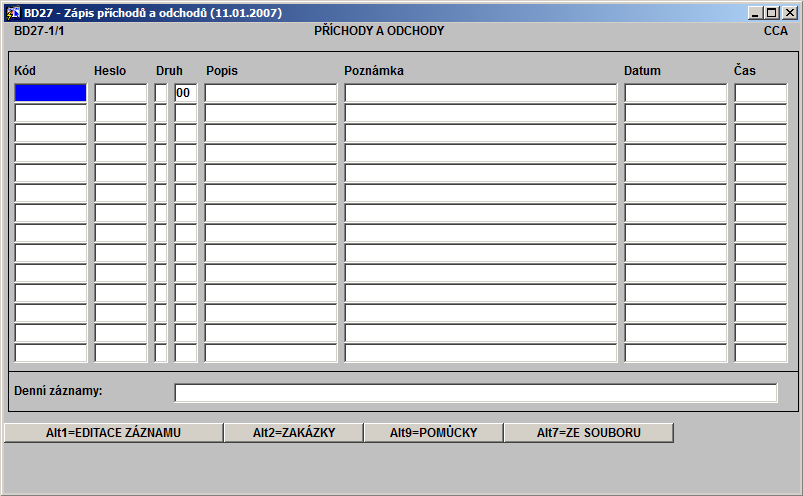
\includegraphics[scale=0.6]{obr/BD27.png}
  \label{}
\end{figure}
+popsat z pohledu uzivatele
\subsection{Výkaz práce}
\begin{figure}[H]
  \centering
  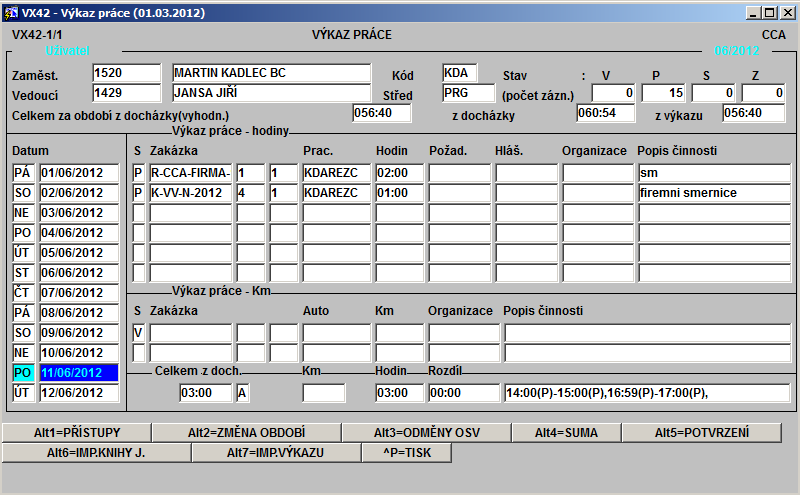
\includegraphics[scale=0.6]{obr/VX42.png}
  \label{}
\end{figure}
+popsat z pohledu uzivatele

\chapter{Analýza}

\section{Architektura}
\subsection{Přímé připojení k databázi}
\subsection{Oracle Database Mobile Server}
Oracle Database Mobile Server 11g - zajistuje synchronizaci mezi Oracle db a mobilnim zarizenim, zamitnuto z licencnich duvodu, mozna by stalo za to to vic prozkoumat a neco o tom napsat
\subsection{Webová služba}

\section{Datová vrstva}
\subsection{Práce s datumem a časem}
Při návrhu datového modelu jsem řešil problém pomocí jakého datového typu vyjadřovat údaj o čase či datu. V Oracle databázi je použit datový typ Date. SQLite databáze nabízí tři způsoby jako ukládat informaci o čase:
\begin{itemize}
\item \textbf{TEXT} podle ISO8601 normy ve formátu "YYYY-MM-DD HH:MM:SS.SSS".
\item \textbf{REAL} podle Juliánského kalendáře, počet dní od poledne 24. Listopadu roku 4714 před kristem (Greenwichského času).
\item \textbf{INTEGER} jako Unix Time, počet sekund 1970-01-01 00:00:00 UTC.
\end{itemize}

\noindent
Pro uložení v SQLite databázi jsem zvolil typ INTEGER. V aplikaci (Android klient, webová služba) jsem se rozhodl reprezentovat časový údaj pomocí primitivního typu long. Měl jsem k tomu řadu dobrých důvodů:
\begin{itemize}
\item odpadá starost s formátem datumu při serializaci a deserializace JSON řetězce
\item snadné porovnávání hodnot pomocí relačních operátorů
\item sníží se počet konverzí v aplikaci (např. pro výpočet pozice pro vykreslení komponenty v UI)
\end{itemize}

Také jsem se ujistil, že rozsah typu long je pro potřeby aplikace dostačující. Srovnání použitých datových typů je znázorněno v tabulce \ref{tab:cas}. 

\begin{table}[H]
\centering
\begin{tabular}{| c | c | c | c |}
\hline
Datový typ &  Minimální hodnota & Maximální hodnota & Přesnost \\ \hline
Oracle Date &   January 1, 4712 BCE  &  December 31, 4712 CE &  sekundy \\ \hline
SQLite INTEGER &    &  &  sekundy \\ \hline
Java long & 2.12.292269055 BC   & 17.8.292278994 AD &  milisekundy \\ \hline
\end{tabular}
\caption{Datové typy reprezentující časový údaj}
\label{tab:cas}
\end{table}

\subsection{Kritika datové vrstvy}
co se mi nelibilo a co bych navrhl jinak a jak, navrh prichody/odchody - jeden radek,
chybi primarni klic - ROWID jako unikatni identifikator, problemy ktere to prinasi,
format casu - problemy s prevodem

\section{Business logika}
existuje někajá možnost převodu formsů do javy - oracle adf - co to je, co to resi, proc to neresi muj problem
\subsection{Triggery}
jen ty, jejichž funkčnost bude muset být implementována.
\begin{itemize}
\item On-Delete, On-Insert, On-Update, Pre-Delete, Pre-Insert, Pre-Update
\item When-Validate-Item
\end{itemize}

\subsection{Databázové balíčky a uložené procedury}

\subsection{Forms knihovny}


\section{Uživatelské rozhraní}
\subsection{LOV}
jaka alternativa v androidu

\chapter{Zabezpečení}

\chapter{Webová služba}

\chapter{Android aplikace}

\section{Funkcionalita}
Na základě analýzy současného systému a potřeb zaměstnanců byla vybrána k implementaci následující funkčnost: 
\paragraph{Docházka}
\begin{itemize}
\item Přehledné zobrazení událostí docházky daného zaměstnance
\item Uživatel má možnost přidávat, ediovat a mazat svoje události
\item Aplikace zajišťuje automatickou synchronzaci těchto údajů s firemní databází
\item Zobrazení poměru typů docházkových událostí za dané období
\end{itemize}
\paragraph{Aktuální přítomnost na pracovišti}
\begin{itemize}
\item Zobrazení seznamu zaměstnanců aktuálně přítomných na pracovišti
\item Uživatel má možnost spravovat seznam svých "oblíbených" zaměstnanců a tento seznam zobrazovat přednostně
\end{itemize}
\paragraph{Výkazy práce}
\begin{itemize}
\item Zobrazení poměru typů zakázek za dané období
\item Zobrazení vývoje vývoje daného typu zakázky v daném období 
\item Možnost zobrazení těchto údajů i za jiné zaměstnance
\end{itemize}

\subsection{Nastavení a konfigurovatelnost}
Aplikace si musí pamatovat údaje nutné pro snadnou obsluhu tzn. uživatelské jméno a heslo, adresu umístění webové služby a tyto údaje jsou konfigurovatelné.\\
Dále aplikace umožní uživateli konfigurovat vzhled některých kompoment, jako je barva typu události v docházce a typu záznamu ve výkazech.

\subsection{Uživatelská přívětivost}
Uživatelské rozhraní aplikace klade důraz na přehlednost, ergonomii a časově efektivní obsluhu.

\section{Architektura}
Android aplikace funguje jako tenký klient, který se připojuje k webové službě. Webová služba používá REST architekturu a přistupuje k samotné databázi.

\begin{figure}[H]
  \centering
  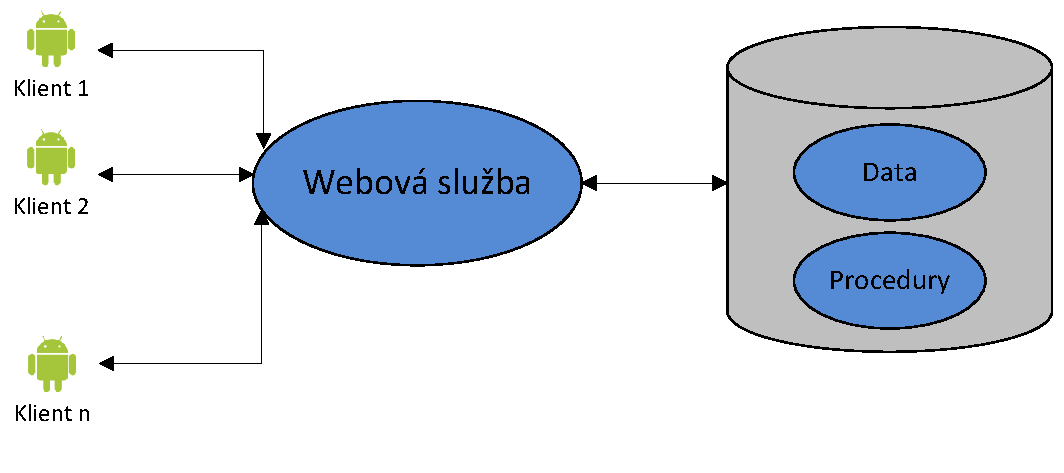
\includegraphics[scale=0.8]{obr/souc_arch2.pdf}
  \label{obr: logo zcu}
\end{figure}

\begin{itemize}
\item Webová služba - Java EE 6, aplikační server GlassFish
\item Databáze - Oracle 10g, obsahuje navíc databázové procedury, které se používají v současných formulářích  
\item Android - obsahuje persistentní úložiště, obsahuje záznamy o docházce, úložiště se bude automaticky synchronizovat ve stavu online s databázovým serverem prostřednictvím webové služby
\end{itemize}
TODO prepsat srozumitelneji
TODO schema komunikace -HHTP, JDBC

\section{Business logika}
prijde to do webove sluzby - duvody

\section{Android komponenty}
\begin{enumerate}
\item komponenty pro sync a auth, provazani s android ucetm
\item CursorLoader
\item Async task
\item  nestandartni UI
\item modifilkace adapterview
\item cutom UI - viewgroup
\end{enumerate}
+ nejaka ukazka konkretniho pouziti

\section{Ukládání dat}

\paragraph{Sdílené preference}\hfill \\ukládá primitivní datové typy ve tvaru klíč-hodnota. Slouží k uložení nastavení specifických pro aplikaci. Toto nastavení může být uloženo jako soukromé, kdy mohou k datům přistupovat pouze aplikace sdílející stejné \emph{Linux user ID}.\\ V aplikaci používám toto úložiště pro nastavení síťového připojení (doména a port webové služby) a barevného nastavení pro typy docházkových událostí.\\
Načtení dat se typicky odehrává v onCreate() metodě aktivity:
\begin{verbatim}
%\begin{lstlisting}
SharedPreferences settings = getSharedPreferences(PREFS_NAME, 
Context.MODE_PRIVATE);
int color = settings.getInt("color", defaultColor);
%\end{lstlisting}
\end{verbatim}
\noindent
Uložení dat se typicky odehrává v onStop() metodě aktivity:
\begin{verbatim}
SharedPreferences settings = getSharedPreferences(PREFS_NAME, 
Context.MODE_PRIVATE);
SharedPreferences.Editor editor = settings.edit();
editor.putInt(("color", userColor);
editor.commit();
\end{verbatim}

\begin{description}
\item [Interní úložiště]\hfill \\
\item [Externí úložiště]\hfill \\
\item [SQLite databáze]\hfill \\
\item [Cloudové úložiště]\hfill \\
\end{description}

\section{SQLite}
je treba resit delku dat napriklad stringu?, dynamic typing

V knihovnách pro Forms aplikace se nachází další kód, který bude nutné přepsat do webové služby.
\section{REST}
\begin{enumerate}
\item REST operace - davkove vs jednotlive
\item REST, tabulka URI, 
\end{enumerate}

\section{Synchronizace}
\begin{enumerate}
\item sync algoritmus - 2 algoritmy (jeden ideální, druhý reálný), srovnání
\item sync architektura - komponenty
\end{enumerate}

\section{Zabezpečení}
-authentikace
Server webové služby je dostupná v síti VPN. Další zabezpečení bude řešeno později...

\section{Zpětná kompatibilita}

\section{Budoucí rozšiřitelnost}

\section{Vytváření grafů}
knihovny, cloudové řešení, vlastní komponenty

\section{Chybové reporty}

\chapter{Testování}

\section{O čem psát...}
\begin{enumerate}
\item popsat IMIS 
\item pripraveno webove sluzby na dalsi mobilni platformy
\item cinnost apliakce online/offline
\item flow diagramy pro ruzne cinnosti
\item pristupova prava
\item uspora pesistentni pameti na strane androida
\item chybove reporty a opravy na aplikaci v ostrem prostredi, obrazek + ukazka
\item jak zjisit zmenu zaznamu, v datech se uklada pouze datum posledni zmeny, nikoli presny cas
\item perioda automatickeho mazani dat
\item budoucnost formsu? 
\item datovy model schema
\end{enumerate}

\section{Zásady pro vypracování}
\begin{enumerate}
\item Prozkoumejte systém IMIS pro evidenci docházky a pracovních výkazů. Vyberte činnosti, které by bylo vhodné implementovat i pro mobilní zařízení.
\item Navrhněte mobilní aplikaci pro platformu Android, které bude obsahovat vybrané funkce z předchozího bodu zadání.
Zvažte aspekty zabezpečení komunikace aplikace se systémem.
\item Implementujte navržené řešení, berte přitom v úvahu možnou rozšiřitelnost o další funkce.
\item Ověřte funkcionalitu vytvořené aplikace.
\end{enumerate}

\appendix
\bibliographystyle{csplainnat}
%\bibliography{bakalarka}

\begin{figure}[H]
  \centering
  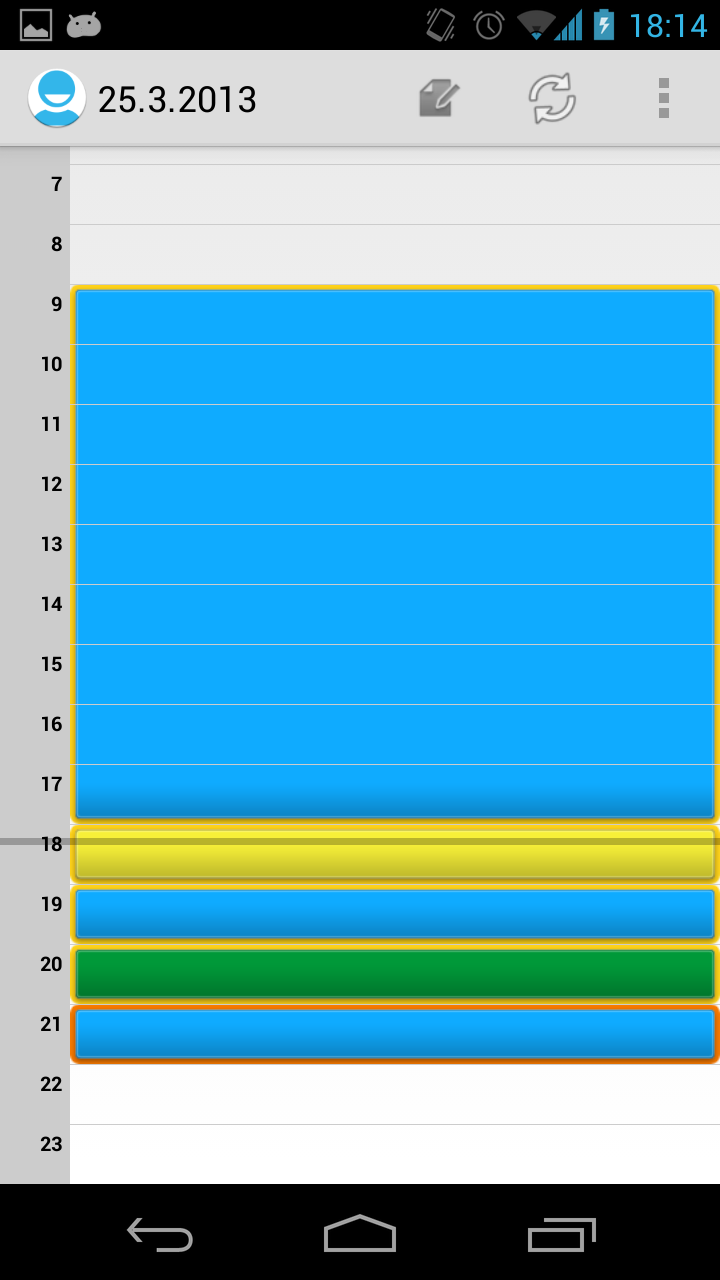
\includegraphics[scale=0.3]{scr/time_doch.png}
  \label{}
\end{figure}

\begin{figure}[H]
  \centering
  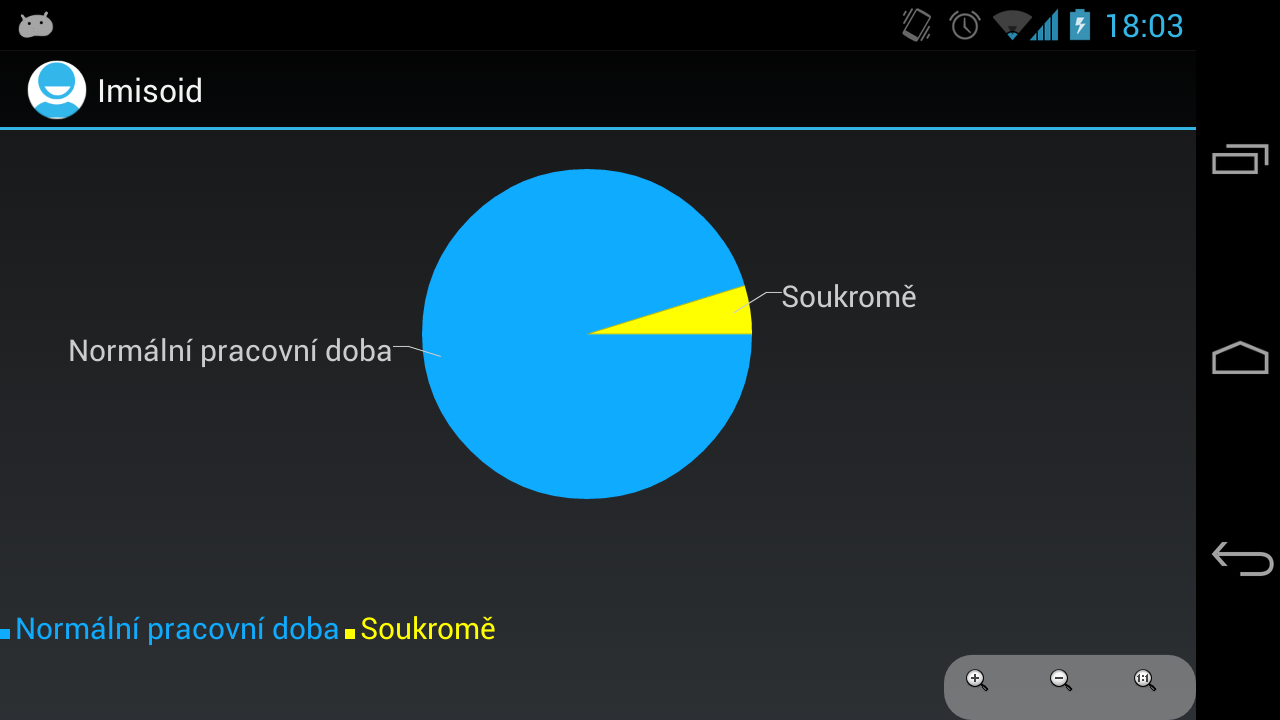
\includegraphics[scale=0.3]{scr/graf_doch.png}
  \label{}
\end{figure}

\begin{figure}[H]
  \centering
  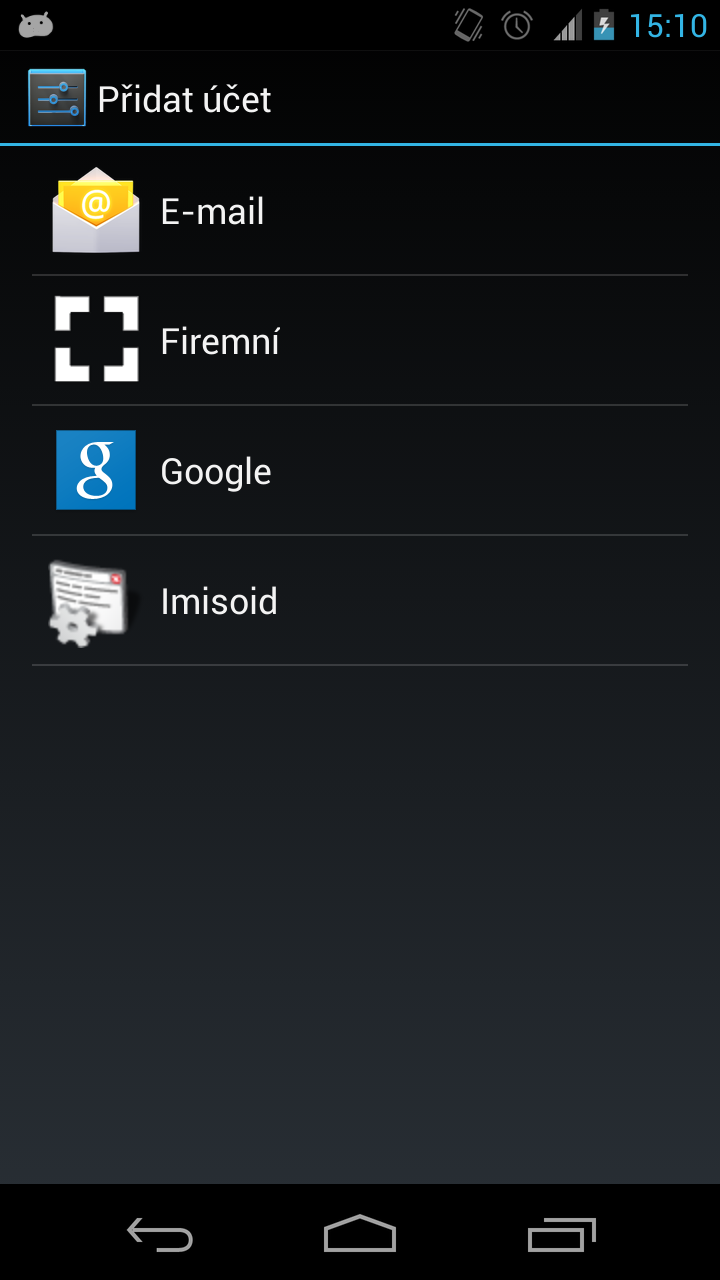
\includegraphics[scale=0.3]{scr/ucet.png}
  \label{}
\end{figure}

\begin{figure}[H]
  \centering
  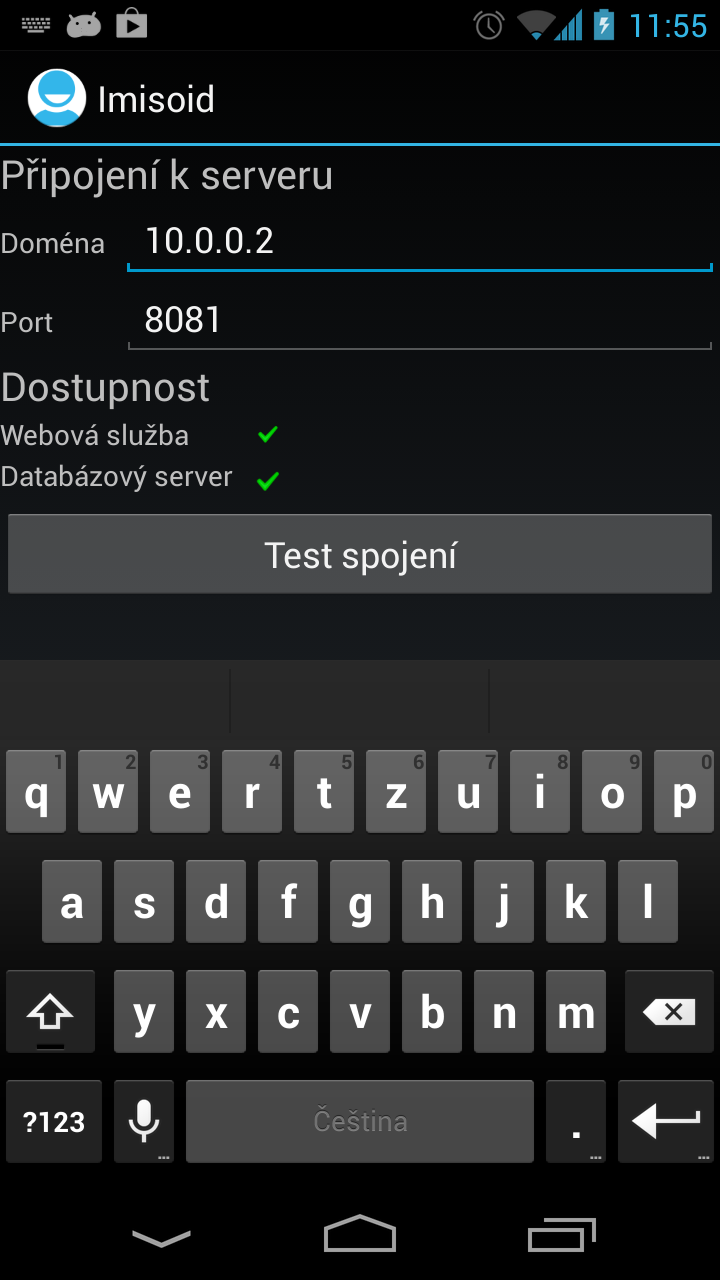
\includegraphics[scale=0.3]{scr/network.png}
  \label{}
\end{figure}
\end{document}
